%!TEX root = ../../main.tex

\section{Linear Temporal Logic}

After a brief introduction to B{\"u}chi Automata and $\omega$-regular languages, concede us to jump to the logic world with Linear Temporal Logic.

Linear Temporal Logic ($\ltl$) is a modal logic interpreted over infinite, discrete and linear ordered time. $\ltl$ can be seen as an extension of propositional logic with the addition of the \textit{next} operator ($\ltlX{\phi}$, i.e. at the next state $\phi$ holds) and the \textit{until} operator ($\ltlU{\phi_1}{\phi_2}$, i.e. $\phi_2$ will eventually hold and $\phi_1$ will hold until then).

\begin{definition}[\cite{geatti-2021-09} The logic $\ltl$]
Let $\Sigma$ be a set of propositions, $\ltl$ formulas are inductively defined as follows:
\begin{flalign*}
\phi := p \; | \; \ltlNeg{\phi} \; | \;  \ltlOr{\phi_1}{\phi_2} \; | \; \ltlX{\phi} \; | \; \ltlU{\phi_1}{\phi_2}
\end{flalign*}
where $p \in \Sigma$.
\end{definition}

Linear temporal logic with Past ($\pastltl$) extends $\ltl$ with the addition of temporal operators that can talk about the past, and it is obtained from $\ltl$ by adding the following past temporal operators: the $\textit{yesterday}$ operator ($\ltlY{\phi}$, i.e. there exists a previous state in which $\phi$ holds); the \textit{weak yesterday} operator ($\ltlZ{\phi}$, i.e. either a previous state does not exist or in the previous state $\phi$ holds); the \textit{since} operator ($\ltlS{\phi_1}{\phi_2}$, i.e. there was a past state where $\phi_2$ held and $\phi_1$ has held since then). 

\begin{definition}[ \cite{geatti-2021-09} The logic $LTL+P$]
Let $\Sigma$ be a set of propositions, $LTL+P$ formulas are inductively defined as follows:
\begin{flalign*}
\phi := p \; &| \; \ltlNeg{\phi} \; | \;  \ltlOr{\phi_1}{\phi_2} \; | \; \ltlAnd{\phi_1}{\phi_2}
\tag{propositional connectives}\\
&|\; \ltlX{\phi} \; | \; \ltlU{\phi_1}{\phi_2} \;
\tag{future temporal operators} \\
&| \; \ltlY{\phi} \; | \; \ltlZ{\phi} \; | \; \ltlS{\phi_1}{\phi_2}
\tag{past temporal operators} \\
\end{flalign*}
where $p \in \Sigma$.
\end{definition}

To simplify writing of formulas, we define following abbreviations:
\begin{enumerate}[label=\roman*.]
    \item true: $\ltlTrue \equiv \ltlOr{\phi}{\ltlNeg{\phi}}$; false: $\ltlFalse \equiv \ltlAnd{\phi}{\ltlNeg{\phi}}$; implication: $\ltlImpl{\phi_1}{\phi_2} \equiv \ltlOr{\ltlNeg{\phi_1}}{\phi_2}$; iff: $\ltlIff{\phi_1}{\phi_2} \equiv \ltlAnd{\ltlImpl{\phi_1}{\phi_2}}{\ltlImpl{\phi_2}{\phi_1}}$;
    \item $\ltlXexp{\phi}{i}$ is $\ltlX{\ltlXexp{\phi}{i-1}}$ if $i > 0$ and $\phi$ if $i=0$;
    \item release: $\ltlR{\phi_1}{\phi_2} \equiv \ltlNeg{(\ltlU{\ltlNeg{\phi_1}}{\ltlNeg{\phi_2}})}$, i.e. either $\phi_2$ is always true, or it will happen that $\phi_1$ is true and in the meantime $\phi_2$ is always true; 
    \item eventually: $\ltlF{\phi} \equiv \ltlU{T}{\phi}$, i.e. $\phi$ will be true eventually;
    \item globally: $\ltlG{\phi} \equiv \ltlNeg{\ltlF{\ltlNeg{\phi}}}$, or $\ltlG{\phi} \equiv \ltlR{\ltlFalse}{\phi}$, i.e. $\phi$ is always true;
    \item trigger: $\ltlT{\phi_1}{\phi_2} \equiv \ltlNeg{(\ltlS{\ltlNeg{\phi_1}}{\ltlNeg{\phi_2}})}$, i.e. either $\phi_2$ was always true in the past, or it is happened that $\phi_1$ was true and in the meantime $\phi_2$ was always true;
    \item once: $\ltlO{\phi} \equiv \ltlS{\ltlTrue}{\phi}$, i.e. $\phi$ was true at least one time in the past; 
    \item historically: $\ltlH{\phi} \equiv \ltlNeg{\ltlO{\ltlNeg{\phi}}}$, i.e. $\phi$ was always true in the past.
\end{enumerate}

We can even make a further distinction starting from $\pastltl$. We say that a $\pastltl$ formula is \textit{pure past} if and only if all temporal operators inside the formula are past operators.
\textit{Full Past LTL} ($\fpltl$) is the fragment of $LTL+P$ that only admits past operators.

Formulas from $\pastltl$ are interpreted over state sequences. A \textit{state sequence} $\sigma = \sequence{\sigma_0,\sigma_1,\dots}$ is an infinite, linearly ordered sequence of states, where each state $\sigma_i$ is a set of proposition letters, that is $\sigma_i \in 2^\Sigma$ for $i \in \Nat$. Given two indices $i,j \in \Nat$ with $i \leq j$, we denote as $\sigma_{[i,j]}$ the interval of $\sigma$ from index $i$ to $j$, that is $\langle \sigma_i,\dots,\sigma_j \rangle$.

To be more precise, let us formalize the semantics of temporal operators we have seen so far plus some additional abbreviations.

\begin{definition}[\cite{geatti-2021-09} $\pastltl$ semantics]
A state-sequence is an infinite sequence $\sigma = \sequence{\sigma_0,\sigma_1,\dots} \in (2^\Sigma)^\omega$ of sets of propositions $\sigma_i \in 2^\Sigma$.
Given a sequence $\sigma$, a position $i\geq 0$ and a formula $\phi$, the satisfaction of $\phi$ by $\sigma$ at $i$, written $\sigma,i \models \phi$, is inductively defined as follows:
\begin{flalign*}
&\sigma,i \models p             &\iff& & & p \in \sigma_i \\
&\sigma,i \models \ltlNeg{\phi} &\iff& & & \sigma,i \not\models \phi \\
&\sigma,i \models \ltlOr{\phi_1}{\phi_2} &\iff& & & \text{$\sigma,i \models \phi_1$ or $\sigma,i \models \phi_2$} \\
&\sigma,i \models \ltlAnd{\phi_1}{\phi_2} &\iff& & & \text{$\sigma,i \models \phi_1$ and $\sigma,i \models \phi_2$} \\
&\sigma,i \models \ltlX{\phi} &\iff& & & \sigma,i+1 \models \phi \\
&\sigma,i \models \ltlY{\phi} &\iff& & & \text{$i>0$ and $\sigma,i-1 \models \phi$} \\
&\sigma,i \models \ltlZ{\phi} &\iff& & & \text{$i=0$ or $\sigma,i-1 \models \phi$} \\
&\sigma,i \models \ltlU{\phi_1}{\phi_2} &\iff& & & \text{$\exists j \geq i$ such that $\sigma,j \models \phi_2$ and} \\
& & & & & \text{$\sigma,k\models \phi_1$ for all $i \leq k < j$} \\
&\sigma,i \models \ltlR{\phi_1}{\phi_2} &\iff& & & \text{either for all $j \geq i$ such that $\sigma,j \models \phi_2$,} \\
& & & & & \text{or $\exists j \geq i$ such that $\sigma,j \models \phi_1$ and} \\
& & & & & \text{$\sigma,k\models \phi_1$ for all $i \leq k \leq j$} \\
&\sigma,i \models \ltlS{\phi_1}{\phi_2} &\iff&&& \text{$\exists j \leq i$ such that $\sigma,j \models \phi_2$ and} \\
& & & & & \text{$\sigma,k\models \phi_1$ for all $j < k \leq i$}
\end{flalign*}
\end{definition}

We say that $\sigma$ satisfies $\phi$, written $\sigma \models \phi$, if and only if $\sigma,0 \models \phi$. In this case we call $\sigma$ a model of $\phi$.

$\ltl$ can also be enriched with bounded temporal operators, such as the \textit{bounded until} $\ltlUbounded{\phi_1}{\phi_2}{[a,b]}$, \textit{bounded eventually} $\ltlFbounded{\phi}{[a,b]} \equiv \ltlUbounded{\ltlTrue}{\phi_2}{[a,b]}$ and \textit{bounded globally} $\ltlGbounded{\phi}{[a,b]} \equiv \ltlNeg{\ltlFbounded{\ltlNeg{\phi}}{[a,b]}}$. We define the bounded until operator as a shortcut for the $\ltl$ formula $\bigvee_{i=a}^{b}(\ltlXexp{\psi_2}{i}\land \bigwedge_{j=0}^{i-1}\ltlXexp{\psi_1}{j})$.
\textit{Full Bounded LTL} ($\fbltl$) is the fragment of LTL that includes only the next and bounded eventually operators.

\textit{Extended Bounded Response LTL} ($\ebrltl$) extends $LTL_{FB}$ by admitting Boolean combinations of the universal unbounded temporal operators release ($\ltlR{}{}$) and globally ($\ltlG{}$).
If we allow using past operators in $\ebrltl$, then we get the $\pastebrltl$ which is defined as follows.

\begin{definition}[\cite{geatti-2020-08} The logic $\ebrltl$]
Let $a,b \in \Nat$. A $\ebrltl$ formula $\chi$ is inductively defined as follows:
\begin{flalign}
&\psi := p \; | \; 
        \ltlNeg{\psi} \; | \; 
        \ltlOr{\psi_1}{\psi_2} \; | \; 
        \ltlX{\psi} \; | \;
        \ltlUbounded{\psi_1}{\psi_2}{[a,b]}
        \tag{Bounded Future Layer} \\
&\phi := \psi \; | \; 
        \ltlAnd{\phi_1}{\phi_2} \; | \; 
        \ltlX{\phi} \; | \; 
        \ltlG{\phi} \; | \; 
        \ltlR{\psi}{\phi}
        \tag{Future Layer} \\
&\chi := \phi \; | \; 
        \ltlOr{\chi_1}{\chi_2} \; | \; 
        \ltlAnd{\chi_1}{\chi_2}
        \tag{Boolean Layer}
\end{flalign}
\end{definition}


\begin{definition}[\cite{geatti-2021-09} The logic $\pastebrltl$]
Let $a,b \in \Nat$, a $\pastebrltl$ formula $\chi$ is inductively defined as follows:
\begin{flalign}
&\eta := p \; | \; 
        \ltlNeg{\eta} \; | \;
        \ltlOr{\eta_1}{\eta_2} \; | \;
        \ltlY{\eta} \; | \;
        \ltlS{\eta_1}{\eta_2}
        \tag{Pure Past Layer} \\
&\psi := \eta \; | \; 
        \ltlNeg{\psi} \; | \; 
        \ltlOr{\psi_1}{\psi_2} \; | \; 
        \ltlX{\psi} \; | \;
        \ltlUbounded{\psi_1}{\psi_2}{[a,b]}
        \tag{Bounded Future Layer} \\
&\phi := \psi \; | \; 
        \ltlAnd{\phi_1}{\phi_2} \; | \; 
        \ltlX{\phi} \; | \; 
        \ltlG{\phi} \; | \; 
        \ltlR{\psi}{\phi}
        \tag{Future Layer} \\
&\chi := \phi \; | \; 
        \ltlOr{\chi_1}{\chi_2} \; | \; 
        \ltlAnd{\chi_1}{\chi_2}
        \tag{Boolean Layer}
\end{flalign}
\end{definition}

Before arguing the advantage to add past temporal operators to $\ebrltl$, we introduce the expressiveness of a temporal logic.
The notion of expressiveness of a temporal logic is an extension of the notion of equivalence of formulas.
We say that two formulas $\phi$ and $\psi$ are equivalent ($\phi \equiv \psi$) if and only if they are satisfied by the same set of state sequences.
A temporal logic $\logic$ is said to be at least as expressive as another temporal logic $\logic'$, if for each formula $\phi \in \logic$, there exists a formula $\psi \in \logic'$ such that $\phi \equiv \psi$.
A temporal logic $\logic$ is said to be less expressive than another temporal logic $\logic'$ if, there exists a formula $\phi \in \logic'$ that for each formula $\psi \in \logic$, $\phi \not\equiv \psi$.
Two temporal logic are equally expressive when they are at least as expressive as each other.

In \cite{geatti-2021-09} has been proved that, without past temporal operators, $\ebrltl$ is less expressive than the safety fragment of $\ltl$. However, we achieve the same expressiveness of the safety fragment of $\ltl$ by adding past temporal operators, becoming a safety language at the same level of other more famous LTL dialects, like $\ltlG{\alpha}$, i.e. formulas starting with \textit{globally} and ending with $\alpha$ is a \textit{pure past formula}, and \textit{Safety-LTL}, i.e. formulas of $\ltl$ without \textit{until} temporal operator and in Negation Normal Form (NNF).
Just to give the general idea of the proof of $\semantics{\ebrltl} \subsetneq \semantics{\ltl} \cap SAFETY$, we can show that the formula $\phi_G := \ltlG{(\ltlOr{p_1}{\ltlG{p_2}})}$ belongs syntactically to Safety-LTL, but it is not expressible by any $\ebrltl$ formula. On the contrary, note that $\phi_G$ is expressible in $\pastebrltl$ since $\phi_G := \ltlG{(\ltlOr{p_1}{\ltlG{p_2}})} \equiv \ltlG{(\ltlImpl{\ltlNeg{p_2}}{\ltlH{p_1}})}$.

\begin{theorem}[\cite{geatti-2021-09} Expressiveness of $\ebrltl$]
$\semantics{\ebrltl} \subsetneq \semantics{\ltl} \cap SAFETY$
\end{theorem}

\begin{theorem}[\cite{geatti-2021-09} Expressiveness of $\pastebrltl$]
$\semantics{\pastebrltl} = \semantics{\ltlG{\alpha}} = \semantics{\text{\textit{Safety-LTL}}} =  \semantics{\ltl} \cap SAFETY$
\end{theorem}

\subsection{Temporal Hierarchy}
Safety and Co-safety properties covers only a subset of all properties expressible by Linear Temporal Logic.
LTL formulas can be divided in classes that form a hierarchy, highlighting the relation among their normal forms defined as Boolean and temporal combinations of full-past formulas. For this reason, whenever we write $\alpha_1$, $\alpha_2$ in this sub-section, we mean two full-past formulas ($\alpha_1,\alpha_2 \in \fpltl$).
Such hierarchy is called Temporal Hierarchy and it was introduced by Manna and Pnueli \cite{pnueli1990}.

Previously we have seen two important type of classes, which are at base of the hierarchy: safety and co-safety properties. 
Safety properties express the fact that "something bad will never happen". An important type of safety properties are invariant properties, which are boolean propositions that must always hold. 
Safety properties are expressible by full-past formulas preceded by a globally operator ($\ltlG{\alpha}$).
Co-safety properties the fact that "a good thing will happen at least one time" and they are expressible by full-past formulas preceded by an eventually operator ($\ltlF{\alpha}$).

The next class of $\ltl$ properties is called obligation class and consists in Boolean combinations of the two classes defined above. 
Its name derived from the fact that its properties impose a conditional obligation ($\ltlOr{\ltlG{\alpha_1}}{\ltlF{\alpha_2}} \equiv \ltlImpl{\ltlF{\alpha_1'}}{\ltlF{\alpha_2}}$ with $\alpha_1' \equiv \ltlNeg{\alpha_1}$), where if something happens, then something else will happen. The normal form of the obligation class is the set of formulas of type $\bigwedge_{i=1}^n(\ltlOr{\ltlG{\alpha_1}}{\ltlF{\alpha_2}})$ for some $n \in \Nat$.

Another formulation for the previous class is the intersection of two other important classes: liveness and persistence. 
\textit{Liveness} expresses properties of type "a good thing will happen infinitely many times" and they are described by formulas of type $\ltlG{\ltlF{\alpha}}$. 
\textit{Persistence} expresses properties of type "a good thing will constantly happen from a certain point on and they are described by formulas of type $\ltlF{\ltlG{\alpha}}$.

Considering the Boolean combinations of liveness and persistence properties, we end up with the reactivity class. A \textit{reactivity} property, like an obligation property, expresses a conditional obligation of the type "if a good thing happens infinitely many times, so does another thing". The normal form of this class comprises all formulas of type $\bigwedge_{i=1}^{n}(\ltlOr{\ltlG{\ltlF{\alpha_1}}}{\ltlF{\ltlG{\alpha_2}}})$, expressible also as $\ltlImpl{\ltlG{\ltlF{\alpha_2'}}}{\ltlG{\ltlF{\alpha_1}}}$ with $\alpha_2' \equiv \ltlNeg{\alpha_2}$, for some $n \in \Nat$. Reactivity class is exactly the set of all $\ltl$ formulas and so they have the same expressiveness.
Actually, there is an entire hierarchy inside the reactivity class, where we define $R(n)$ for some $n \in \Nat$ as the classes of formulas with a fixed number $n$ of conjunctions.
Moreover, it is been proved that $\semantics{R(n)} \subsetneq \semantics{R(n+1)}$ for each $n \in \Nat$.


\begin{figure}[!htp]
    \centering
    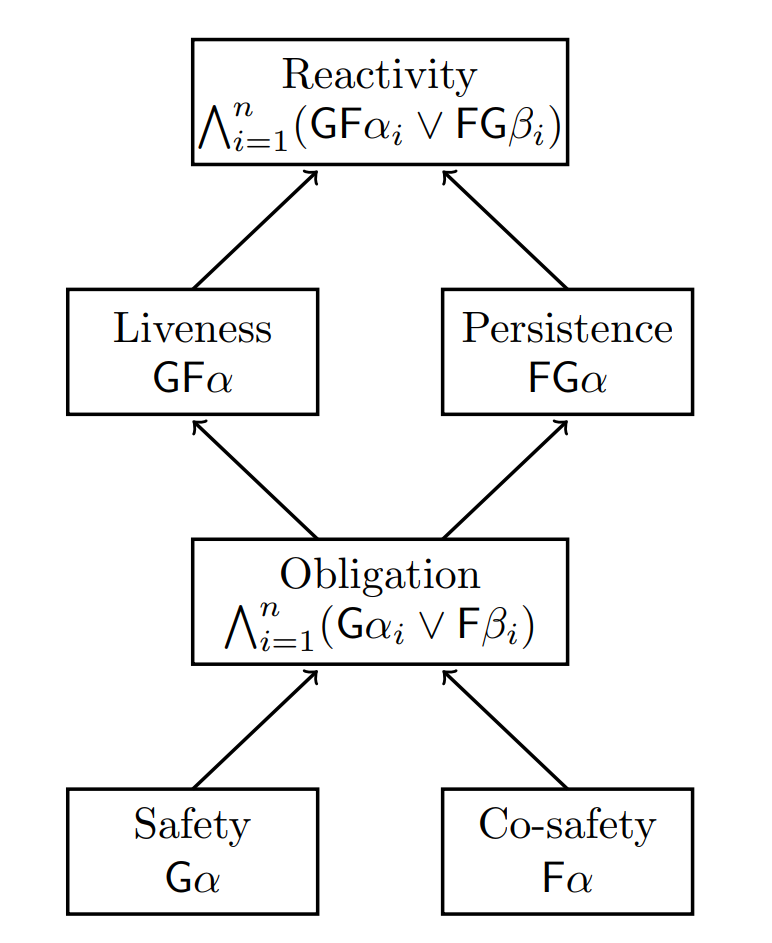
\includegraphics[width=0.4\linewidth]{figures/temporal-hierarchy.png}
    \caption{\cite{pnueli1990} Temporal Hierarchy describing the relation among temporal classes along with their normal forms. The arrows represent the inclusions between the classes.}
    \label{fig:temporal-hierarchy}
\end{figure}
